\documentclass[aspectratio=169,11pt]{beamer}
\usetheme{metropolis}
\usepackage{booktabs}
\usepackage{graphicx}
\usepackage{xcolor}
\usepackage{tikz}
\usetikzlibrary{arrows.meta, positioning, shapes.geometric}
\usepackage{appendixnumberbeamer}
\graphicspath{{../figures/shapes/talk/}{../figures/shapes/}}

\definecolor{vizblue}{HTML}{2A78D6}
\definecolor{vizorange}{HTML}{EB6834}
\definecolor{vizgrey}{HTML}{8A8A8A}
\definecolor{vizaqua}{HTML}{1BAF7A}
\definecolor{vizyellow}{HTML}{EDA100}
\setbeamercolor{progress bar}{fg=vizblue}
\setbeamercolor{title separator}{fg=vizblue}
\setbeamercolor{alerted text}{fg=vizorange}
\metroset{numbering=fraction, progressbar=frametitle}

\title{RTF: Real-Time Fingerprints Experimentation}
\subtitle{}
\author{Mat Madhavacheril, Nayan Patel}
\date{October 2026}

\begin{document}

\maketitle

% ---------------------------------------------------------------------------
\begin{frame}{The problem}
  \centering
  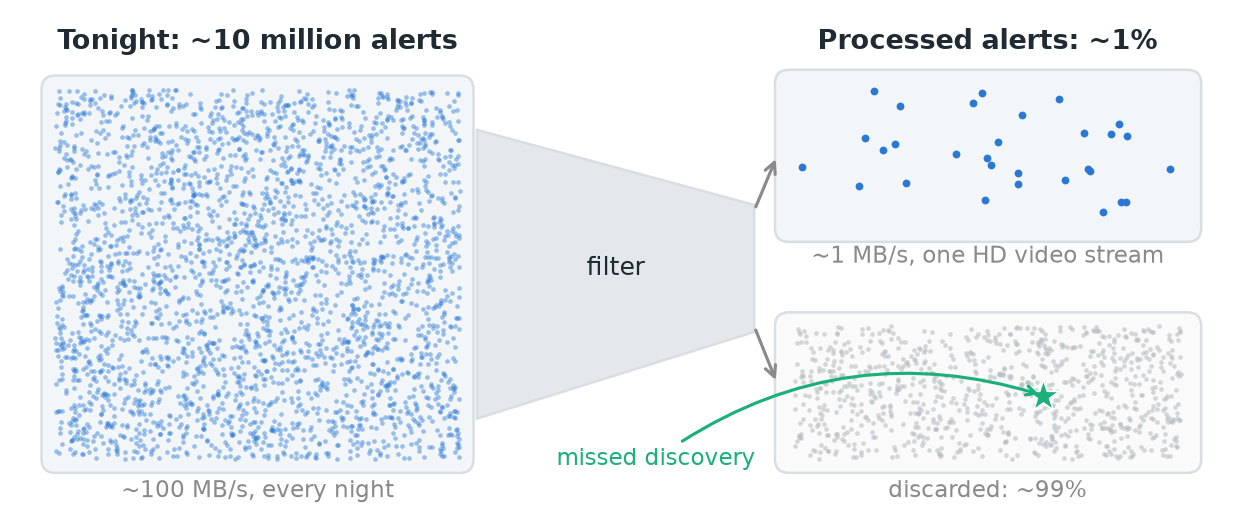
\includegraphics[width=0.78\textwidth]{talk_alert_flood.png}
  \vspace{0.2em}
  \begin{itemize}
    \item LSST will issue $\sim$10 million alerts every night.
    \item Each one: the light curve, a $63{\times}63$ pixel cutout triplet,
      and metadata.
    \item Brokers can only use a small subset, and the filtration leads to missed
      discoveries.
  \end{itemize}
\end{frame}

% ---------------------------------------------------------------------------
\begin{frame}{Inputs: the cutout triplet}
  \centering
  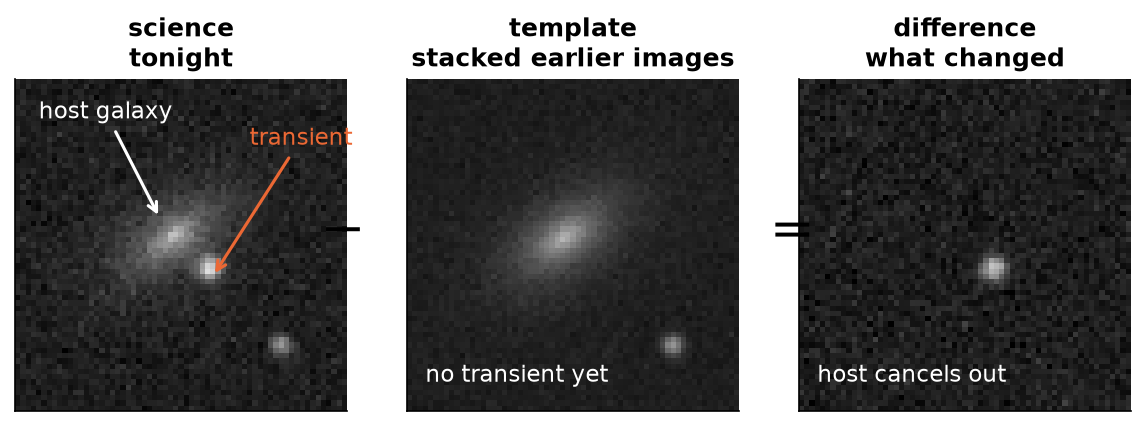
\includegraphics[width=0.47\textwidth]{talk_triplet_explained.png}
  \vspace{-0.5em}
  \begin{columns}[T]
    \column{0.48\textwidth}
    \footnotesize
    \begin{itemize}
      \item \textbf{Science:} current observation, $63{\times}63$ pixels
        around the candidate. Captures the transient, host, neighbours, and the sky.
      \item \textbf{Template:} images of the sky before the transient.
      \item \textbf{Difference:} what changed between the template and science.
    \end{itemize}
    \column{0.5\textwidth}
    \footnotesize
    \textbf{Why all three?}
    \begin{itemize}
      \item The template is sharper than the science, so PSF scaling blurs the sharper template image before subtraction against the science. 
      \item The template can give context about the host.
      \item Science + template can expose bad subtractions.
    \end{itemize}
  \end{columns}
\end{frame}

% ---------------------------------------------------------------------------
\begin{frame}{Inputs: the light curve}
  \begin{columns}[T]
    \column{0.58\textwidth}
    \centering
    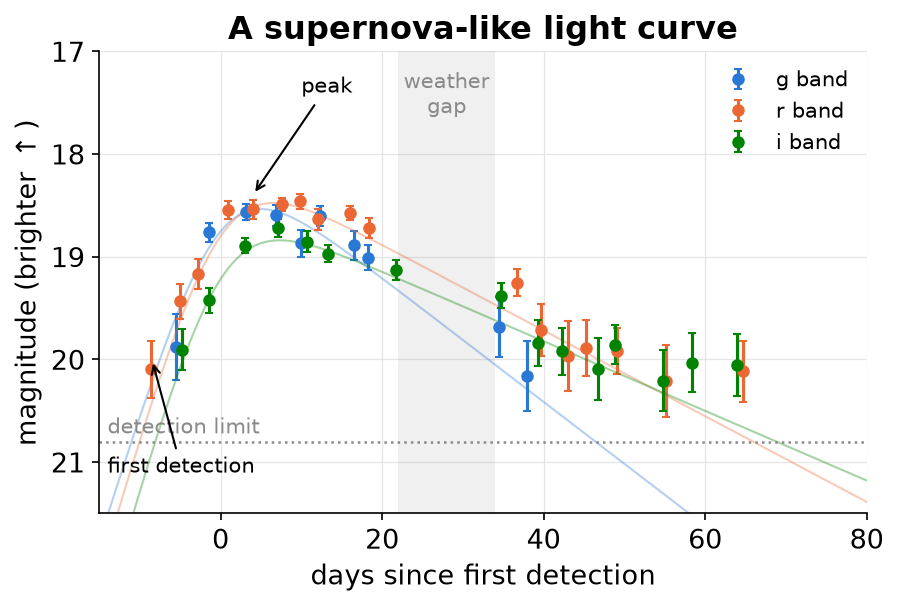
\includegraphics[height=0.72\textheight]{talk_light_curve.png}
    \column{0.42\textwidth}
    \footnotesize
    Brightness vs.\ time in three bands, sampled at uneven intervals when the survey records.
    \vspace{0.3em}

    \textbf{Datapoints:}
    \vspace{0.1em}

    \begin{tabular}{@{}ll@{}}
      \toprule
      time since first detection & $\log(1{+}\Delta t)$ \\
      gap since previous one     & $\log(1{+}\delta t)$ \\
      flux, flux error           & $\log$ \\
      filter                     & g / r / i flag \\
      \bottomrule
    \end{tabular}
    \vspace{0.2em}

    Variable in length (depends on number of observations from the survey). \textbf{Switched off for this experiment.}
  \end{columns}
\end{frame}

% ---------------------------------------------------------------------------
\begin{frame}{Inputs: the metadata}
  About 30 numbers the pipeline has already computed for every alert to give context. Examples:
  \begin{itemize}
    \item nearest catalogued source: distance, brightness, star or galaxy
    \item how point-like the detection is
    \item the survey's own real-vs-bogus score
    \item how many detections so far
  \end{itemize}
  \vspace{0.5em}
  \textbf{Also switched off for this experiment.}
\end{frame}

% ---------------------------------------------------------------------------
\begin{frame}{The idea}
  \centering
  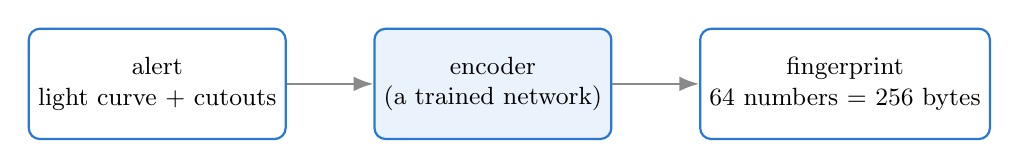
\begin{tikzpicture}[
      box/.style={draw=vizblue, thick, rounded corners, minimum height=1.4cm,
                  minimum width=2.6cm, align=center, font=\small},
      arr/.style={-{Latex[length=2.5mm]}, thick, vizgrey}]
    \node[box] (a) {alert\\light curve + cutouts};
    \node[box, right=1.1cm of a, fill=vizblue!10] (e) {encoder\\(a trained network)};
    \node[box, right=1.1cm of e] (z) {fingerprint\\64 numbers = 256 bytes};
    \draw[arr] (a) -- (e);
    \draw[arr] (e) -- (z);
  \end{tikzpicture}
  \vspace{0.8em}

  \textbf{What we can do with fingerprints}
  \begin{itemize}
    \item Supervised learning (classify).
    \item Unsupervised learning (cluster).
  \end{itemize}
\end{frame}

% ---------------------------------------------------------------------------
\begin{frame}{Solving for out-of-distribution}
  \centering
  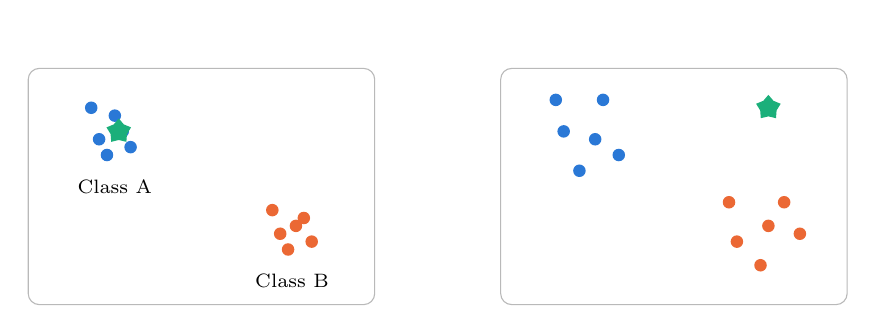
\begin{tikzpicture}[x=1cm, y=1cm, dot/.style={circle, inner sep=1.6pt}]
    % left: tidy clusters, unknown lands inside one
    \node[font=\small\bfseries] at (2.2,3.4) {};
    \draw[rounded corners, draw=vizgrey!60] (0,0) rectangle (4.4,3.0);
    \foreach \p in {(0.9,2.1),(1.1,2.4),(1.3,2.0),(0.8,2.5),(1.2,2.2),(1.0,1.9)}
      \node[dot, fill=vizblue] at \p {};
    \foreach \p in {(3.2,0.9),(3.5,1.1),(3.3,0.7),(3.6,0.8),(3.1,1.2),(3.4,1.0)}
      \node[dot, fill=vizorange] at \p {};
    \node[star, star points=5, fill=vizaqua, inner sep=2.2pt] at (1.15,2.2) {};
    \node[font=\scriptsize] at (1.1,1.5) {Class A};
    \node[font=\scriptsize] at (3.35,0.3) {Class B};
    \node[font=\scriptsize, vizaqua] at (2.3,2.6) {};
    % right: looser clusters, unknown sits alone
    \begin{scope}[xshift=6cm]
      \node[font=\small\bfseries] at (2.2,3.4) {};
      \draw[rounded corners, draw=vizgrey!60] (0,0) rectangle (4.4,3.0);
      \foreach \p in {(0.8,2.2),(1.3,2.6),(1.5,1.9),(0.7,2.6),(1.2,2.1),(1.0,1.7)}
        \node[dot, fill=vizblue] at \p {};
      \foreach \p in {(3.0,0.8),(3.6,1.3),(3.3,0.5),(3.8,0.9),(2.9,1.3),(3.4,1.0)}
        \node[dot, fill=vizorange] at \p {};
      \node[star, star points=5, fill=vizaqua, inner sep=2.2pt] at (3.4,2.5) {};
      \node[font=\scriptsize, vizaqua] at (3.3,2.0) {};
    \end{scope}
  \end{tikzpicture}
  \vspace{0.5em}
  \begin{itemize}
    \item The question we try to address: can an encoder trained on known classes also flag unknown ones?
    \item In other words: can we detect a new transient class without ever having seen one?
  \end{itemize}
\end{frame}

% ---------------------------------------------------------------------------
\begin{frame}{Simple experiment: circles vs.\ squares}
  \centering
  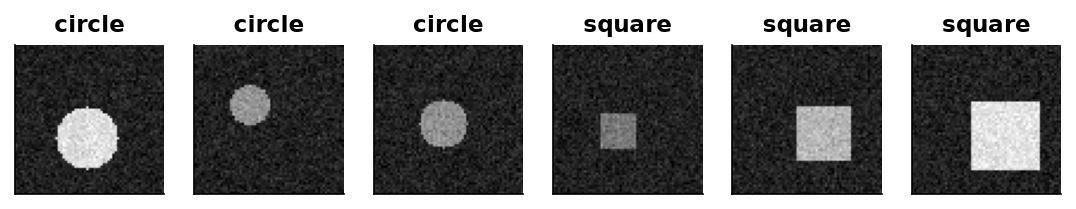
\includegraphics[width=0.9\textwidth]{talk_stamps_row.png}
  \vspace{0.6em}
  \begin{itemize}
    \item Light-curve input switched off: the fingerprint depends only on the cutout.
    \item Synthetic stamps: circles and squares of equal area, random size, position
      and brightness, plus noise. 
  \end{itemize}
\end{frame}

% ---------------------------------------------------------------------------
\begin{frame}{Two ways to build the image encoder}
  \centering
  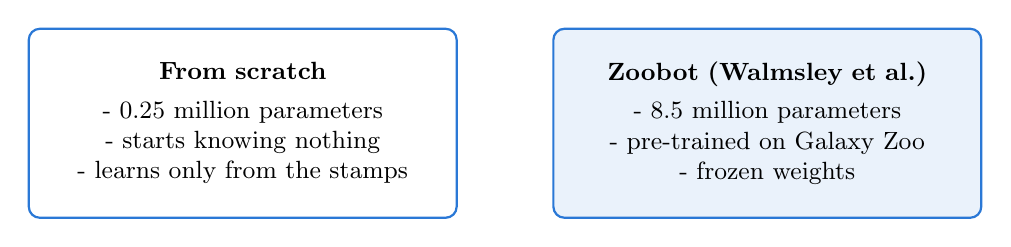
\begin{tikzpicture}[
      box/.style={draw=vizblue, thick, rounded corners, minimum height=2.4cm,
                  text width=5.2cm, align=center, font=\small}]
    \node[box] (a) {\textbf{From scratch}\\[0.3em]
      - 0.25 million parameters\\ - starts knowing nothing\\ - learns only from the stamps};
    \node[box, right=1.2cm of a, fill=vizblue!10] (b) {\textbf{Zoobot (Walmsley et al.)}\\[0.3em]
      - 8.5 million parameters\\ - pre-trained on Galaxy Zoo \\
      - frozen weights};
  \end{tikzpicture}
\end{frame}

% ---------------------------------------------------------------------------
\begin{frame}{Encoder 1: the from-scratch CNN}
  \centering
  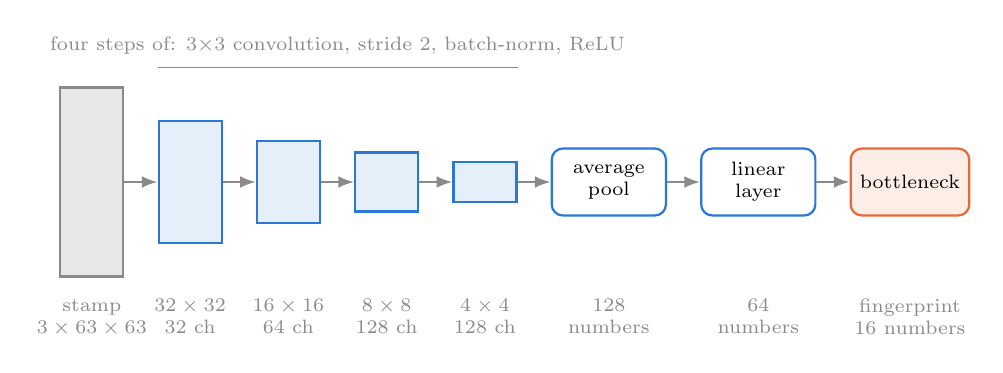
\begin{tikzpicture}[
      fm/.style={draw=vizblue, thick, fill=vizblue!12, minimum width=0.8cm},
      vec/.style={draw=vizblue, thick, fill=white, rounded corners,
                  minimum width=1.45cm, minimum height=0.85cm, align=center,
                  font=\scriptsize},
      lab/.style={font=\scriptsize, text=vizgrey, align=center, anchor=north},
      arr/.style={-{Latex[length=2mm]}, vizgrey, thick},
      node distance=0.42cm]
    \node[fm, minimum height=2.4cm, fill=vizgrey!20, draw=vizgrey] (in) {};
    \node[fm, minimum height=1.55cm, right=of in] (c1) {};
    \node[fm, minimum height=1.05cm, right=of c1] (c2) {};
    \node[fm, minimum height=0.75cm, right=of c2] (c3) {};
    \node[fm, minimum height=0.5cm, right=of c3] (c4) {};
    \node[vec, right=of c4] (pool) {average\\pool};
    \node[vec, right=of pool] (lin) {linear\\layer};
    \node[vec, right=of lin, fill=vizorange!12, draw=vizorange] (z) {bottleneck};
    \coordinate (base) at ([yshift=-0.15cm]in.south);
    \node[lab] at (in |- base) {stamp\\$3\times63\times63$};
    \node[lab] at (c1 |- base) {$32\times32$\\32 ch};
    \node[lab] at (c2 |- base) {$16\times16$\\64 ch};
    \node[lab] at (c3 |- base) {$8\times8$\\128 ch};
    \node[lab] at (c4 |- base) {$4\times4$\\128 ch};
    \node[lab] at (pool |- base) {128\\numbers};
    \node[lab] at (lin |- base) {64\\numbers};
    \node[lab] at (z |- base) {fingerprint\\16 numbers};
    \foreach \a/\b in {in/c1, c1/c2, c2/c3, c3/c4, c4/pool, pool/lin, lin/z}
      \draw[arr] (\a) -- (\b);
    \draw[vizgrey] ([yshift=1.45cm]c1.west) -- ([yshift=1.45cm]c4.east)
      node[midway, above=0.05cm, font=\scriptsize, text=vizgrey]
      {four steps of: $3{\times}3$ convolution, stride 2, batch-norm, ReLU};
  \end{tikzpicture}
  \vspace{0.2em}
  \small
  \begin{itemize}
    \item  $\sim$0.25 million parameters, all trained on from random starting
      values using the stamps (\textcolor{vizblue}{blue} = trained here).
    \item After pooling, the readout (linear + bottleneck) is identical for both
      encoders. Maps the pool of features to a 16-number fingerprint.
  \end{itemize}
\end{frame}

% ---------------------------------------------------------------------------
\begin{frame}{Encoder 2: Zoobot, frozen}
  \centering
  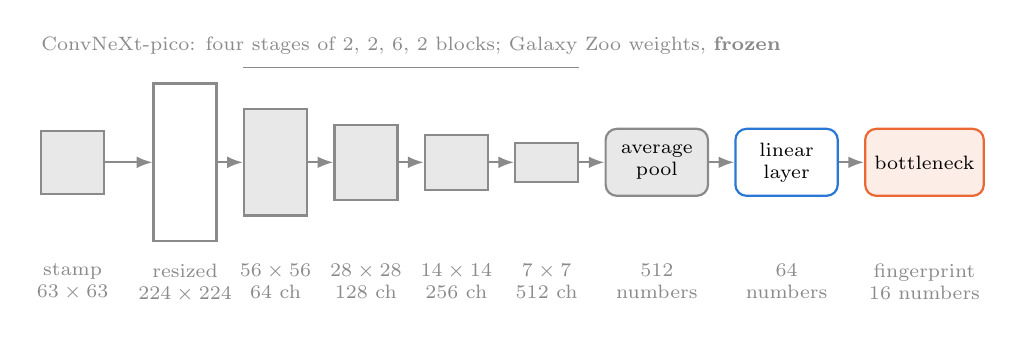
\begin{tikzpicture}[
      fm/.style={draw=vizgrey, thick, fill=vizgrey!20, minimum width=0.8cm},
      vec/.style={draw=vizblue, thick, fill=white, rounded corners,
                  minimum width=1.3cm, minimum height=0.85cm, align=center,
                  font=\scriptsize},
      frz/.style={draw=vizgrey, thick, fill=vizgrey!20, rounded corners,
                  minimum width=1.3cm, minimum height=0.85cm, align=center,
                  font=\scriptsize},
      lab/.style={font=\scriptsize, text=vizgrey, align=center, anchor=north},
      arr/.style={-{Latex[length=2mm]}, vizgrey, thick},
      node distance=0.32cm]
    \node[fm, minimum height=0.8cm] (in) {};
    \node[fm, minimum height=2.0cm, right=0.6cm of in, fill=white] (up) {};
    \node[fm, minimum height=1.35cm, right=of up] (s1) {};
    \node[fm, minimum height=0.95cm, right=of s1] (s2) {};
    \node[fm, minimum height=0.7cm, right=of s2] (s3) {};
    \node[fm, minimum height=0.5cm, right=of s3] (s4) {};
    \node[frz, right=of s4] (pool) {average\\pool};
    \node[vec, right=of pool] (lin) {linear\\layer};
    \node[vec, right=of lin, fill=vizorange!12, draw=vizorange] (z) {bottleneck};
    \coordinate (base) at ([yshift=-0.15cm]up.south);
    \node[lab] at (in |- base) {stamp\\$63\times63$};
    \node[lab] at (up |- base) {resized\\$224\times224$};
    \node[lab] at (s1 |- base) {$56\times56$\\64 ch};
    \node[lab] at (s2 |- base) {$28\times28$\\128 ch};
    \node[lab] at (s3 |- base) {$14\times14$\\256 ch};
    \node[lab] at (s4 |- base) {$7\times7$\\512 ch};
    \node[lab] at (pool |- base) {512\\numbers};
    \node[lab] at (lin |- base) {64\\numbers};
    \node[lab] at (z |- base) {fingerprint\\16 numbers};
    \foreach \a/\b in {in/up, up/s1, s1/s2, s2/s3, s3/s4, s4/pool, pool/lin, lin/z}
      \draw[arr] (\a) -- (\b);
    \draw[vizgrey] ([yshift=1.2cm]s1.west) -- ([yshift=1.2cm]s4.east)
      node[midway, above=0.05cm, font=\scriptsize, text=vizgrey]
      {ConvNeXt-pico: four stages of 2, 2, 6, 2 blocks; Galaxy Zoo weights, \textbf{frozen}};
  \end{tikzpicture}
  \vspace{0.2em}
  \small
  \begin{itemize}
    \item $\sim$8.5 million parameters, pre-trained to reproduce galaxy morphology on millions of galaxies. \textcolor{vizgrey}{Grey} = frozen, used exactly as published.
    \item The stamp is upsampled because the network expects $224{\times}224$ inputs.
    \item We train only the \textcolor{vizblue}{blue} readout ($\sim$35k parameters).
  \end{itemize}
\end{frame}


% ---------------------------------------------------------------------------
\begin{frame}{Result 1: from-scratch classification}
  \begin{columns}[T]
    \column{0.5\textwidth}
    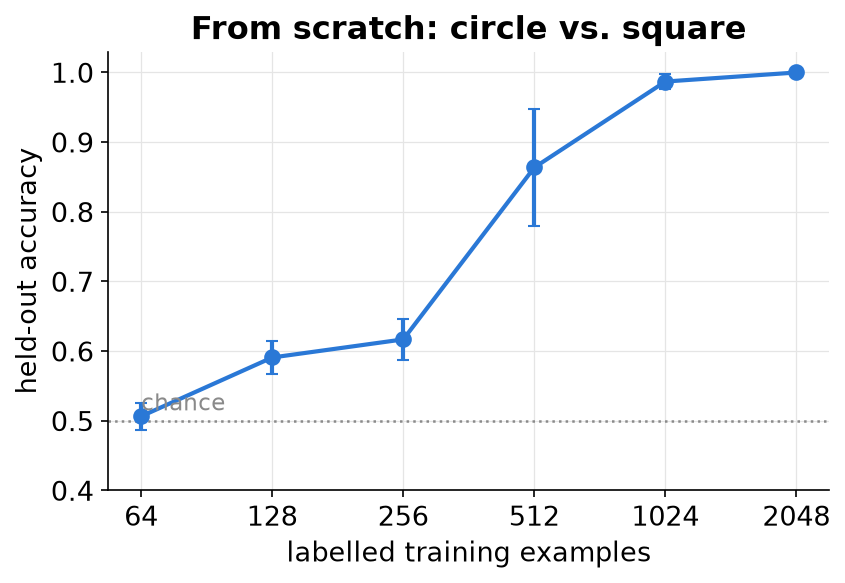
\includegraphics[width=\textwidth]{talk_data_efficiency.png}
    \column{0.5\textwidth}
    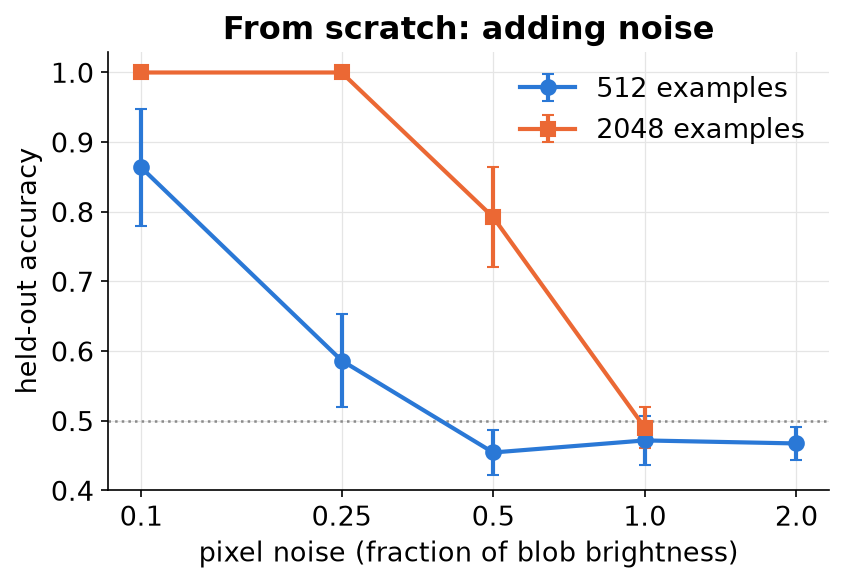
\includegraphics[width=\textwidth]{talk_noise.png}
  \end{columns}
  \begin{itemize}
    \item 256 examples: 62\,\%. About 1000 examples: 99\,\%.
    \item Add modest noise and 512 examples is no longer enough, but 2048 fixes it.
    \item Takeaway: from-scratch compression works well, but requires lots of data (which may not exist for rare classes).
  \end{itemize}
\end{frame}

% ---------------------------------------------------------------------------
\begin{frame}{Result 2: Zoobot classification}
  \begin{columns}[T]
    \column{0.55\textwidth}
    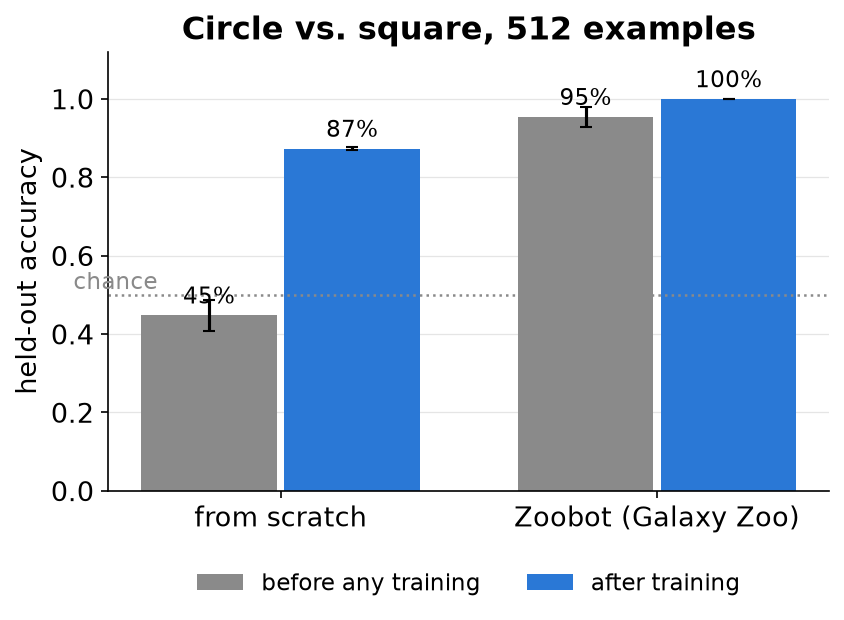
\includegraphics[width=\textwidth]{talk_backbone.png}
    \column{0.43\textwidth}
    \vspace{1em}
    \begin{itemize}
      \item ``Before'' means a random readout after the frozen Zoobot encoder (zero training). ``after'' means the readout has been trained to classify circles vs.\ squares.
      \item Takeaway: Zoobot is already a capable encoder and requires far less data to accurately classify. 
    \end{itemize}
  \end{columns}
\end{frame}

% ---------------------------------------------------------------------------
\begin{frame}{The discovery test: out-of-distribution shapes}
  \centering
  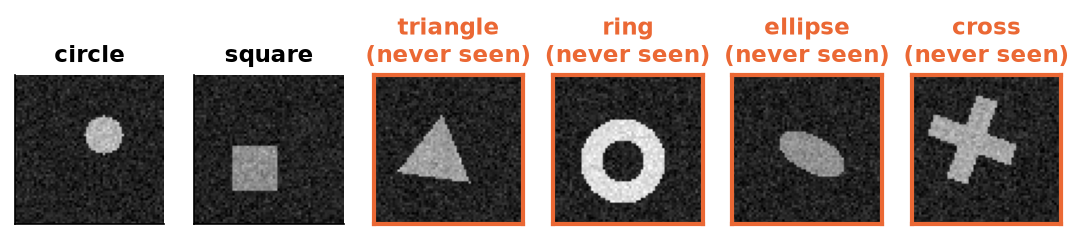
\includegraphics[width=0.8\textwidth]{talk_novel_row.png}
  \vspace{0.2em}
  \begin{itemize}
    \item Train on circles and squares only. Then show four new shapes. We want to know: 
    \begin{enumerate}
      \item Are the fingerprint latents for the new shapes far from the existing circles and squares we trained on?
      \item If we group the fingerprint latents blindly, do the new shapes get their own groups?
    \end{enumerate}
  \end{itemize}
\end{frame}

% ---------------------------------------------------------------------------
\begin{frame}{Metrics used}
  \begin{columns}[T]
    \column{0.5\textwidth}
    \textbf{New-shape detection} \hfill {\footnotesize\textcolor{vizgrey}{no labels used}}
    \footnotesize
    \begin{enumerate}
      \item Encode the 2048 circle/square \emph{training} stamps.
      \item Encode the 1536 held-out stamps (256 per shape, six shapes).
      \item For each held-out fingerprint, find its 5 nearest training
        fingerprints. The mean of those 5 distances is its novelty score.
      \item We measure the chance that a random new-shape stamp outscores a random held-out circle or square (50\,\% useless, 100\,\% perfect).
    \end{enumerate}

    \column{0.5\textwidth}
    \textbf{Six-shape separability} \hfill {\footnotesize\textcolor{vizgrey}{labels used}}
    \footnotesize
    \begin{enumerate}
      \item Take the same 1536 held-out fingerprints, now with all six true labels.
      \item Fit a 6-way logistic regression. 
      \item Accuracy = fraction of the 1536 predicted correctly.
        Chance $= 1/6 \approx 17\,\%$.
      \item Determines if the class information is present in the fingerprint. 
    \end{enumerate}
  \end{columns}
\end{frame}

% ---------------------------------------------------------------------------
\begin{frame}{Result 3: from-scratch vs.\ Zoobot for new-shape detection}
  \centering
  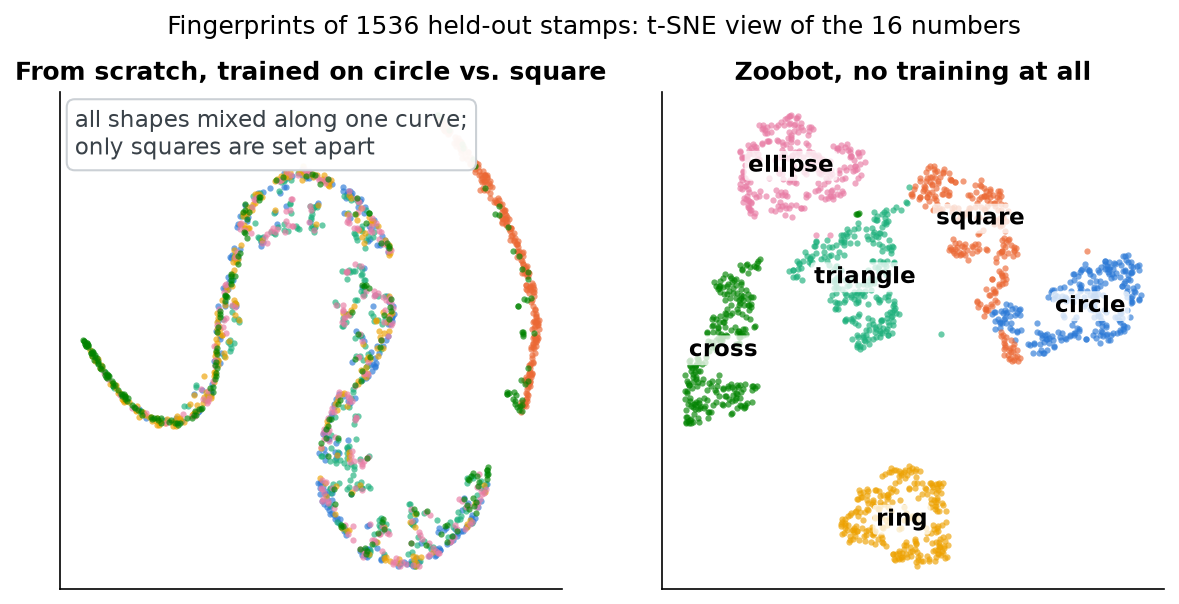
\includegraphics[width=0.7\textwidth]{talk_tsne_pair.png}
  \begin{columns}[T]
    \column{0.5\textwidth}
    \small
    \textbf{From scratch:} new-shape detection 68\,\%, six-shape separability 43\,\%.
    Triangles, rings and ellipses are all grouped with circles. 1 effective dimension. 
    \column{0.5\textwidth}
    \small
    \textbf{Zoobot, no training:} detection 99.8\,\%, separability 99.5\,\%.
    New classes form their own islands. 5 effective dimensions. 
  \end{columns}
\end{frame}

% ---------------------------------------------------------------------------
\begin{frame}{Result 4: teaching Zoobot to classify collapses the fingerprint}
  \begin{columns}[T]
    \column{0.62\textwidth}
    \centering
    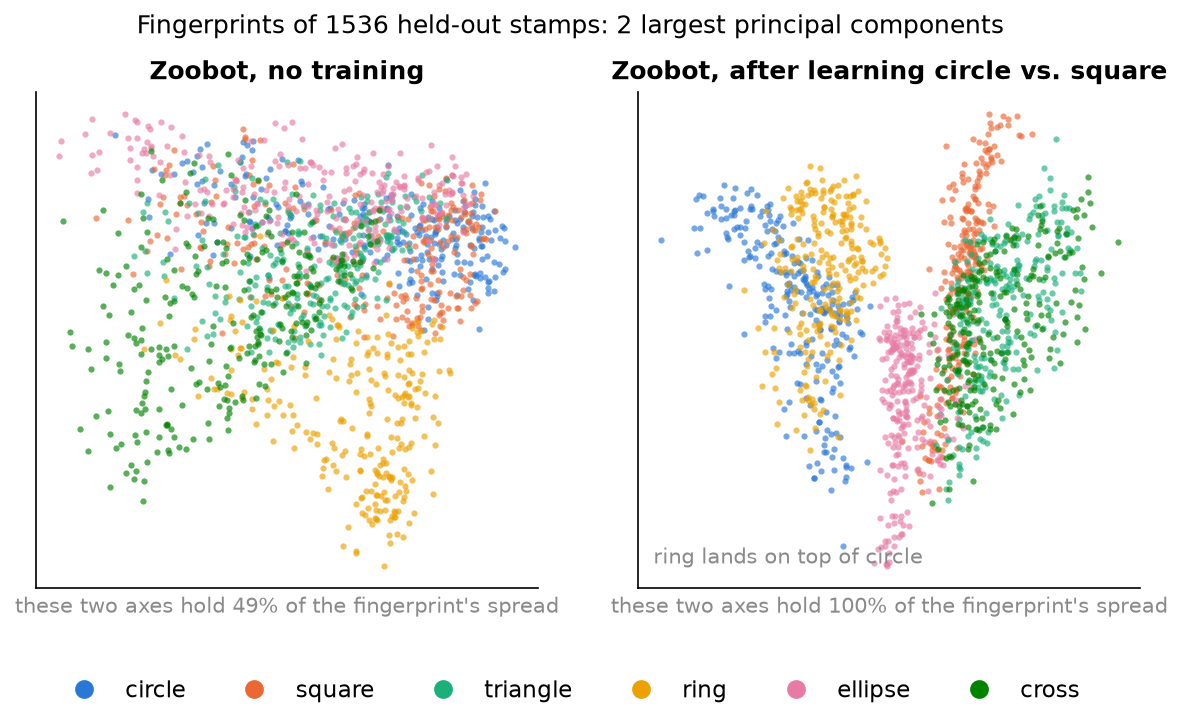
\includegraphics[width=\textwidth]{talk_pca_pair.png}
    \column{0.38\textwidth}
    \vspace{0.6em}
    \begin{itemize}
      \item We fine-tune the Zoobot readout to classify circles vs.\ squares.
      \item Once the readout learns circle vs.\ square, the fingerprint collapses onto
        a line (1 effective dimension).
      \item Triangles, rings and ellipses are all projected onto the same line as
        circles.
      \item Six-shape separability: 99.5\,\% $\to$ 85\,\%.
    \end{itemize}
  \end{columns}
\end{frame}

% ---------------------------------------------------------------------------
\begin{frame}{Summary}
  \textbf{Key takeaways}
  \begin{enumerate}
    \item Use a Galaxy Zoo pre-trained encoder for cutouts. From-scratch isn't viable for rare class classification. 
    \item Pretraining substantially beats from-scratch for out-of-distribution. 
    \item A reconstruction-type objective is helpful during training to prevent  collapse.
  \end{enumerate}
  \textbf{Limitations / Future directions}
  \begin{itemize}
    \item The shapes in our experiment were easy, and real data will likely behave differently.
    \item We're still not sure if Galaxy Zoo specifically is producing the results, or if ordinary 
    ImageNet-pretrained networks can achieve similar performance. 
    \item Additional fine-tuning methods can be explored (e.g., unfreezing parts of the encoder). 
  \end{itemize}
\end{frame}

% ---------------------------------------------------------------------------
\appendix

\begin{frame}{Appendix}
  \centering
  \footnotesize
  \begin{tabular}{@{}lcccc@{}}
    \toprule
    fingerprint built by
      & \shortstack{separability\\(with labels)}
      & \shortstack{new-shape\\detection}
      & \shortstack{blind\\grouping}
      & \shortstack{dims\\used} \\
    \midrule
    untrained small network     & 0.23 & 0.55 & 0.00 & 3.3 \\
    small network, classify     & 0.43 & 0.68 & 0.28 & 1.0 \\
    small network, reconstruct  & 0.34 & 0.75 & 0.01 & 5.2 \\
    small network, both         & 0.44 & 0.68 & 0.23 & 2.7 \\
    Zoobot, no training         & \textbf{0.995} & \textbf{0.998} & 0.54 & 4.8 \\
    Zoobot, classify            & 0.85 & 0.96 & 0.54 & 1.0 \\
    Zoobot, both                & 0.97 & 0.97 & \textbf{0.62} & 1.4 \\
    \bottomrule
  \end{tabular}
  \vspace{0.5em}

  2048 training stamps, 256 held-out stamps per shape.
\end{frame}

\end{document}
